\documentclass[aspectratio=169]{beamer}
\usepackage[utf8]{inputenc}
\usepackage{xcolor}
\usepackage{tikz}
\usepackage{listings}
\usepackage{lstautogobble}
\usepackage{wdqs}
\usepackage{hyperref}

\title{Querying Linked Data with SPARQL and the Wikidata Query Service}
\author{Lucas Werkmeister}
\date{2019-12-27}

\usetheme{Rochester}
\beamertemplatenavigationsymbolsempty
\setbeamertemplate{footline}[text line]{%
  \parbox{0.3\linewidth}{%
    \insertshortauthor%
  }%
  \hfill%
  \parbox{0.37\linewidth}{%
    \url{https://tinyurl.com/36c3-wdqs}%
  }%
  \hfill%
  \insertframenumber/20%
}


\usetikzlibrary{shapes}
\usetikzlibrary{shapes.multipart}

\colorlet{talk}{blue!50!black}
\colorlet{room}{red!50!black}

\tikzset{
  % node options
  iri/.style={ellipse,draw},
  literal/.style={rectangle,draw},
  var/.style={ellipse,dashed,draw},
  varTalk/.style={var,text=talk},
  varRoom/.style={var,text=room},
  result/.style={iri,thick},
  resultTalk/.style={result,text=talk},
  resultRoom/.style={result,text=room},
  varliteral/.style={var,literal},
  % path options
  predicate/.style={->,auto},
  predicate bidi/.style={predicate,bend left=5,inner sep=0.25mm},
  % matrix options
  row sep=7mm,
  column sep=15mm,
}

\lstset{language=[wdqs]sparql,autogobble}

\newcommand{\Esszimmer}{\node[iri] (Esszimmer) {Esszimmer};}
\newcommand{\Kueche}{\node[iri] (Kueche) {Küche};}
\newcommand{\thistalk}{\node[iri] (this talk) {this talk};}
\newcommand{\livequerying}{\node[iri] (live querying) {live querying};}
\newcommand{\WikipakaWG}{\node[iri] (WikipakaWG) {WikipakaWG};}
\newcommand{\TagEinsNoon}{\node[literal] (Tag 1 noon) {2019-12-27T\\12:00:00+0100};}
\newcommand{\Congress}{\node[iri] (36C3) {36C3};}
\newcommand{\Klimawahlen}{\node[iri] (Klimawahlen) {Klimawahlen};}
\newcommand{\ChaosWestStage}{\node[iri] (Chaos-West Stage) {Chaos-West\\Stage};}
\newcommand{\ChaosWest}{\node[iri] (Chaos West) {Chaos West};}

\newcommand{\Vlivequerying}{\node[varTalk] (live querying) {\rlap{?talk}\hphantom{live querying}};}
\newcommand{\Vthistalk}{\node[varTalk] (this talk) {\rlap{?talk}\hphantom{this talk}};}
\newcommand{\VEsszimmer}{\node[varRoom] (Esszimmer) {\rlap{?room}\hphantom{Esszimmer}};}
\newcommand{\Rlivequerying}{\node[resultTalk] (live querying) {live querying};}
\newcommand{\Rthistalk}{\node[resultTalk] (this talk) {this talk};}
\newcommand{\REsszimmer}{\node[resultRoom] (Esszimmer) {Esszimmer};}

\newcommand{\thistalklivequerying}{\draw[predicate bidi] (this talk) to node {is followed by} (live querying);}
\newcommand{\livequeryingthistalk}{\draw[predicate bidi] (live querying) to node {follows} (this talk);}
\newcommand{\thistalkEsszimmer}{\draw[predicate,bend left] (this talk) to node {happens in} (Esszimmer);}
\newcommand{\livequeryingEsszimmer}{\draw[predicate,swap] (live querying) to node {happens in} (Esszimmer);}
\newcommand{\EsszimmerWikipakaWG}{\draw[predicate,bend left=5] (Esszimmer) to node [pos=.6,inner sep=0] {is part of} (WikipakaWG);}

\newcommand{\Twitter}[1]{\href{https://twitter.com/#1}{@#1}}
\newcommand{\Mastodon}[2]{\href{https://#2/@#1}{@#1@#2}}
\newcommand{\wwiki}[1]{\href{https://w.wiki/#1}{w.wiki/#1}}

\begin{document}

\frame{\titlepage}

\begin{frame}[fragile]
  \frametitle{An example graph}
  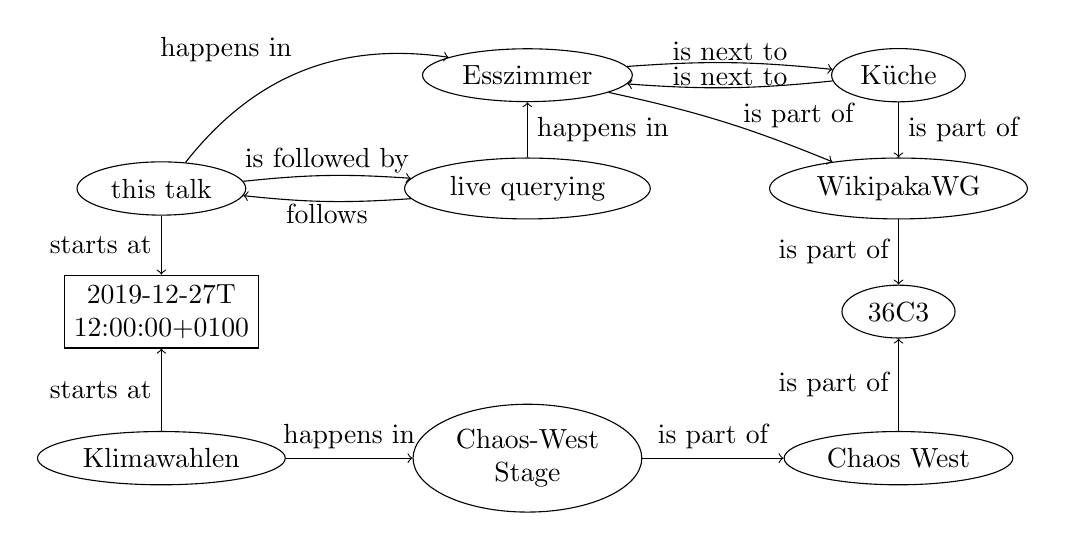
\begin{tikzpicture}[
      every text node part/.style={align=center},
    ]
    \matrix {
      & \Esszimmer & \Kueche \\
      \thistalk & \livequerying & \WikipakaWG \\
      \TagEinsNoon & & \Congress \\
      \Klimawahlen & \ChaosWestStage & \ChaosWest \\
    };
    \thistalklivequerying
    \livequeryingthistalk
    \thistalkEsszimmer
    \livequeryingEsszimmer
    \draw[predicate bidi] (Esszimmer) to node {is next to} (Kueche);
    \draw[predicate bidi,swap] (Kueche) to node {is next to} (Esszimmer);
    \EsszimmerWikipakaWG
    \draw[predicate] (Kueche) to node {is part of} (WikipakaWG);
    \draw[predicate,swap] (WikipakaWG) to node {is part of} (36C3);
    \draw[predicate,swap] (this talk) to node {starts at} (Tag 1 noon);
    \draw[predicate] (Klimawahlen) to node {starts at} (Tag 1 noon);
    \draw[predicate] (Klimawahlen) to node {happens in} (Chaos-West Stage);
    \draw[predicate] (Chaos-West Stage) to node {is part of} (Chaos West);
    \draw[predicate] (Chaos West) to node {is part of} (36C3);
  \end{tikzpicture}
\end{frame}

\begin{frame}[fragile]
  \setlength{\parskip}{5mm}
  \frametitle{Example questions}
  Which talk follows this one?

  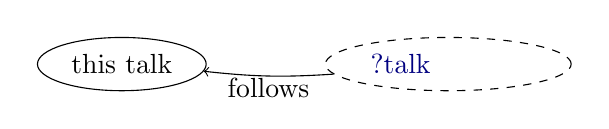
\begin{tikzpicture}
    \matrix {
      \thistalk & \Vlivequerying \\
    };
    \livequeryingthistalk
  \end{tikzpicture}

  Matching triple:

  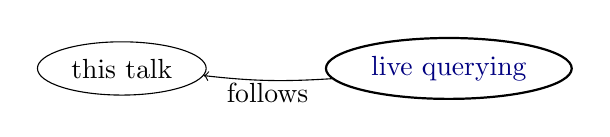
\begin{tikzpicture}
    \matrix {
      \thistalk & \Rlivequerying \\
    };
    \livequeryingthistalk
  \end{tikzpicture}
\end{frame}

\begin{frame}[fragile]
  \setlength{\parskip}{5mm}
  \frametitle{Example questions}
  Same question, phrased differently:
  Which talk is this one followed by?
  This talk is followed by which one?

  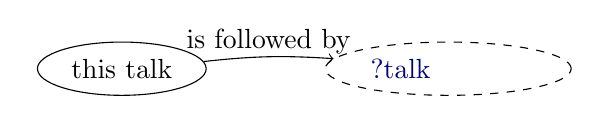
\begin{tikzpicture}
    \matrix {
      \thistalk & \Vlivequerying \\
    };
    \thistalklivequerying
  \end{tikzpicture}

  Matching triple:

  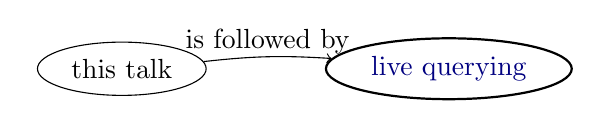
\begin{tikzpicture}
    \matrix {
      \thistalk & \Rlivequerying \\
    };
    \thistalklivequerying
  \end{tikzpicture}
\end{frame}

\begin{frame}[fragile]
  \frametitle{Example questions}
  Which talk happens in Esszimmer?

  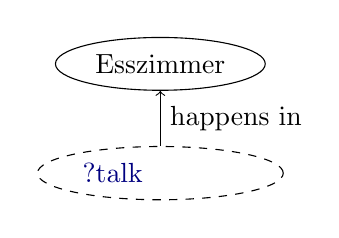
\begin{tikzpicture}
    \matrix {
      \Esszimmer \\
      \Vlivequerying \\
    };
    \livequeryingEsszimmer
  \end{tikzpicture}

  Matching triples:

  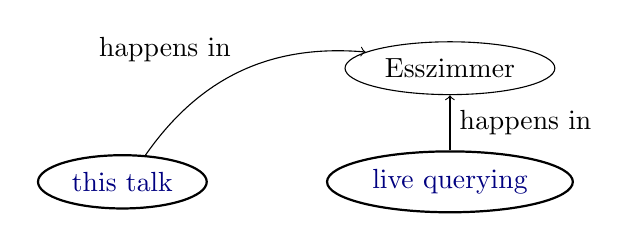
\begin{tikzpicture}
    \matrix {
      & \Esszimmer \\
      \Rthistalk & \Rlivequerying \\
    };
    \thistalkEsszimmer
    \livequeryingEsszimmer
  \end{tikzpicture}
\end{frame}

\begin{frame}[fragile]
  \frametitle{Example questions}
  Which talks happen in the WikipakaWG?
  That is, which talks happen in a room that’s part of the WikipakaWG?

  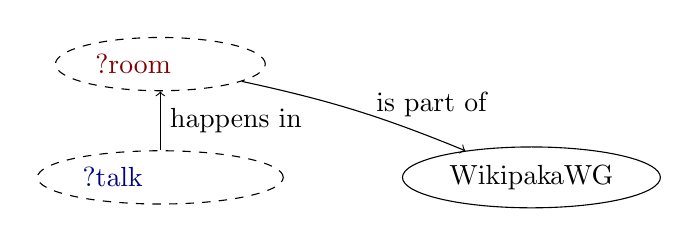
\begin{tikzpicture}
    \matrix {
      \VEsszimmer & \\
      \Vlivequerying & \WikipakaWG \\
    };
    \livequeryingEsszimmer
    \EsszimmerWikipakaWG
  \end{tikzpicture}

  Matching triples:

  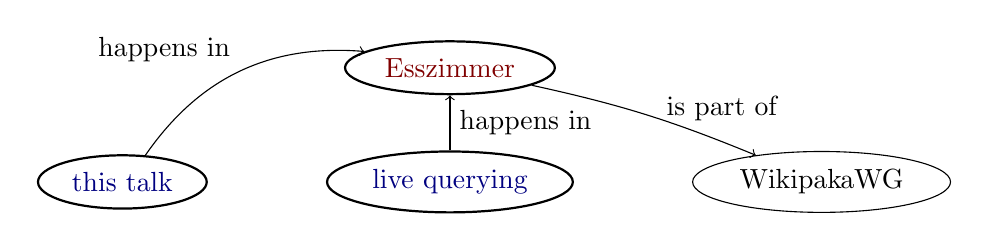
\begin{tikzpicture}
    \matrix {
      & \REsszimmer & \\
      \Rthistalk & \Rlivequerying & \WikipakaWG \\
    };
    \thistalkEsszimmer
    \livequeryingEsszimmer
    \EsszimmerWikipakaWG
  \end{tikzpicture}
\end{frame}

\begin{frame}[fragile]
  \frametitle{SPARQL}
  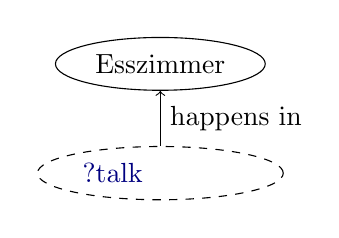
\begin{tikzpicture}
    \matrix {
      \Esszimmer \\
      \Vlivequerying \\
    };
    \livequeryingEsszimmer
  \end{tikzpicture}

  might translate into:

  \begin{lstlisting}
    SELECT * WHERE {
      ?talk 36c3:happensIn 36c3:Esszimmer.
    }
  \end{lstlisting}

  The \lstinline{36c3:} \emph{prefix} clarifies which Esszimmer we’re talking about.
\end{frame}

\begin{frame}[fragile]
  \frametitle{SPARQL}
  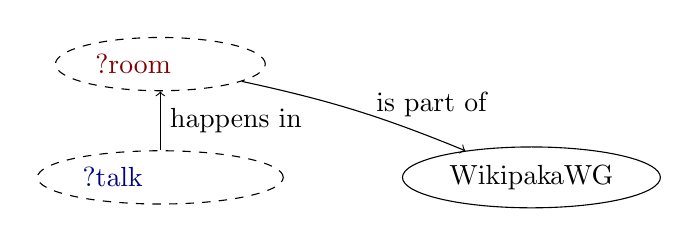
\begin{tikzpicture}
    \matrix {
      \VEsszimmer & \\
      \Vlivequerying & \WikipakaWG \\
    };
    \livequeryingEsszimmer
    \EsszimmerWikipakaWG
  \end{tikzpicture}

  might translate into:

  \begin{lstlisting}
    SELECT * WHERE {
      ?talk 36c3:happensIn ?room.
      ?room 36c3:isPartOf 36c3:WikipakaWG.
    }
  \end{lstlisting}
\end{frame}

\begin{frame}[fragile]
  \frametitle{SPARQL}
  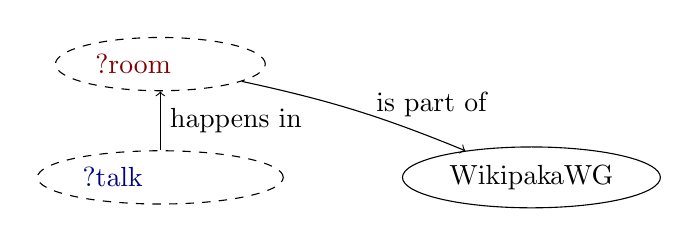
\begin{tikzpicture}
    \matrix {
      \VEsszimmer & \\
      \Vlivequerying & \WikipakaWG \\
    };
    \livequeryingEsszimmer
    \EsszimmerWikipakaWG
  \end{tikzpicture}

  might also translate into:

  \begin{lstlisting}
    SELECT ?talk WHERE {
      ?talk 36c3:happensIn [
        schema:isPartOf 36c3:WikipakaWG
      ].
    }
  \end{lstlisting}
\end{frame}

\begin{frame}[fragile]
  \setlength{\parskip}{5mm}
  \frametitle{Example queries}
  Which software is written in Bash?
  \pause

  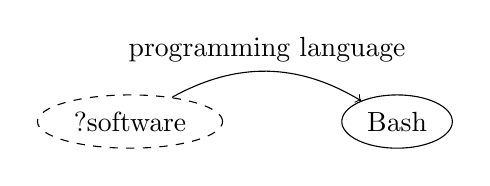
\begin{tikzpicture}
    \matrix {
      \node[var] (software) {?software}; & \node[iri] (Bash) {Bash}; \\
    };
    \draw[predicate,bend left] (software) to node {programming language} (Bash);
  \end{tikzpicture}
  \pause

  \begin{lstlisting}
    SELECT ?software WHERE {
      ?software wdt:P277 wd:Q189248.
    }
  \end{lstlisting}
\end{frame}

\begin{frame}[fragile]
  \setlength{\parskip}{5mm}
  \frametitle{Example queries}
  Who was born at sea?
  \pause

  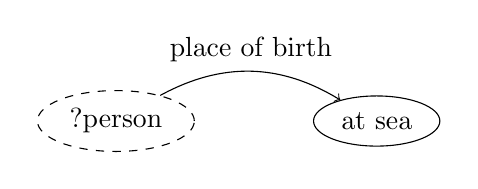
\begin{tikzpicture}
    \matrix {
      \node[var] (person) {?person}; & \node[iri] (at sea) {at sea}; \\
    };
    \draw[predicate,bend left] (person) to node {place of birth} (at sea);
  \end{tikzpicture}
  \pause

  \begin{lstlisting}
    SELECT ?person WHERE {
      ?person wdt:P19 wd:Q55438959.
    }
  \end{lstlisting}
\end{frame}

\begin{frame}[fragile]
  \setlength{\parskip}{5mm}
  \frametitle{Example queries}
  Which places are located on the White Elster?
  \pause

  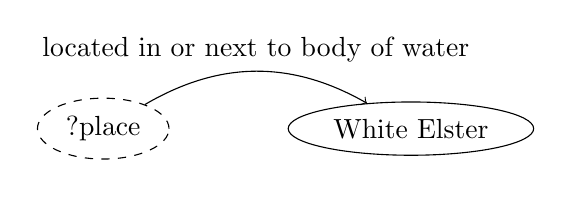
\begin{tikzpicture}
    \matrix {
      \node[var] (place) {?place}; & \node[iri] (White Elster) {White Elster}; \\
    };
    \draw[predicate,bend left] (place) to node {located in or next to body of water} (White Elster);
  \end{tikzpicture}
  \pause

  \begin{lstlisting}
    SELECT ?place WHERE {
      ?place wdt:P206 wd:Q44729.
    }
  \end{lstlisting}
\end{frame}

\begin{frame}[fragile]
  \setlength{\parskip}{5mm}
  \frametitle{Example queries}
  Where does The Neverending Story take place?
  \pause

  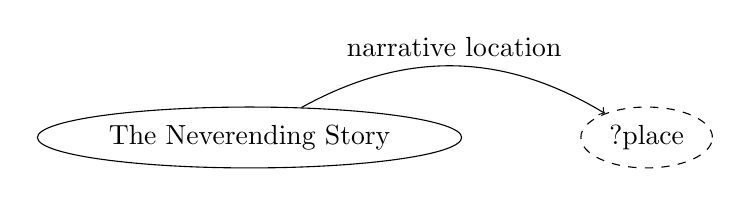
\begin{tikzpicture}
    \matrix {
      \node[iri] (The Neverending Story) {The Neverending Story}; & \node[var] (place) {?place}; \\
    };
    \draw[predicate,bend left] (The Neverending Story) to node {narrative location} (place);
  \end{tikzpicture}
  \pause

  \begin{lstlisting}
    SELECT ?place WHERE {
      wd:Q463108 wdt:P840 ?place.
    }
  \end{lstlisting}
\end{frame}

\begin{frame}[fragile]
  \frametitle{Example queries}
  Which popes had children?
  \pause

  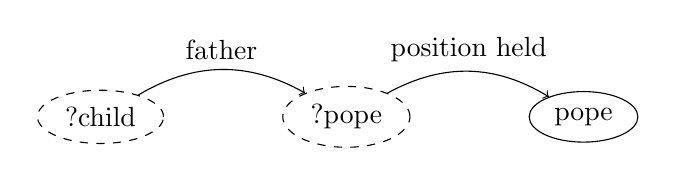
\begin{tikzpicture}
    \matrix {
      \node[var] (child) {?child}; & \node[var] (pope) {?pope}; & \node[iri] (Pope) {pope}; \\
    };
    \draw[predicate,bend left] (child) to node {father} (pope);
    \draw[predicate,bend left] (pope) to node {position held} (Pope);
  \end{tikzpicture}
  \pause

  \begin{lstlisting}
    SELECT ?pope ?child WHERE {
      ?child wdt:P22 ?pope.
      ?pope wdt:P39 wd:Q19546.
    }
  \end{lstlisting}
\end{frame}

\begin{frame}[fragile]
  \frametitle{Example queries}
  Which popes had children?
  \pause

  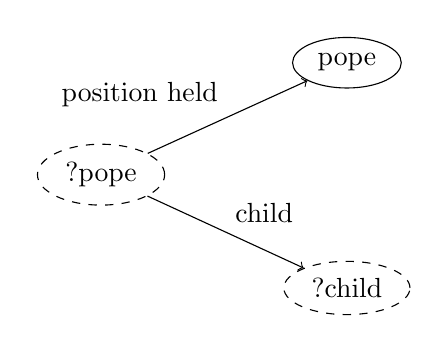
\begin{tikzpicture}
    \matrix {
      & \node[iri] (Pope) {pope}; \\
      \node[var] (pope) {?pope}; & \\
      & \node[var] (child) {?child}; \\
    };
    \draw[predicate] (pope) to node {position held} (Pope);
    \draw[predicate] (pope) to node {child} (child);
  \end{tikzpicture}
  \pause

  \begin{lstlisting}
    SELECT ?pope ?child WHERE {
      ?pope wdt:P39 wd:Q19546;
            wdt:P40 ?child.
    }
  \end{lstlisting}
\end{frame}

\begin{frame}[fragile]
  \frametitle{Example queries}
  Which Microsoft software runs on Linux?
  \pause

  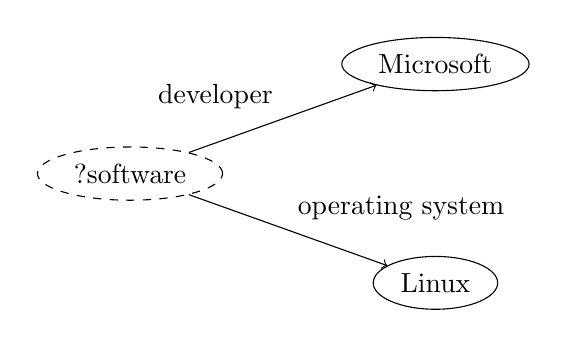
\begin{tikzpicture}
    \matrix {
      & \node[iri] (Microsoft) {Microsoft}; \\
      \node[var] (software) {?software}; & \\
      & \node[iri] (Linux) {Linux}; \\
    };
    \draw[predicate] (software) to node {developer} (Microsoft);
    \draw[predicate] (software) to node {operating system} (Linux);
  \end{tikzpicture}
  \pause

  \begin{lstlisting}
    SELECT ?software WHERE {
      ?software wdt:P178 wd:Q2283;
                wdt:P306 wd:Q388.
    }
  \end{lstlisting}
\end{frame}

\begin{frame}[fragile]
  \frametitle{Example queries}
  What are some compositions for organ and orchestra?
  \pause

  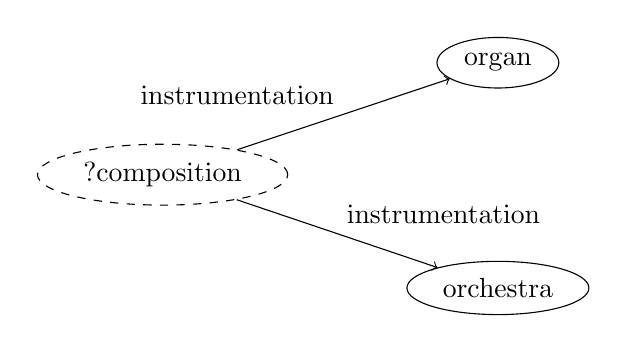
\begin{tikzpicture}
    \matrix {
      & \node[iri] (organ) {organ}; \\
      \node[var] (composition) {?composition}; & \\
      & \node[iri] (orchestra) {orchestra}; \\
    };
    \draw[predicate] (composition) to node {instrumentation} (organ);
    \draw[predicate] (composition) to node {instrumentation} (orchestra);
  \end{tikzpicture}
  \pause

  \begin{lstlisting}
    SELECT ?composition WHERE {
      ?composition wdt:P870 wd:Q1444, wd:Q42998.
    }
  \end{lstlisting}
\end{frame}

\begin{frame}[fragile]
  \frametitle{Example queries}
  Which Nazi party members later received the Order of Merit of the Federal Republic of Germany?
  \pause

  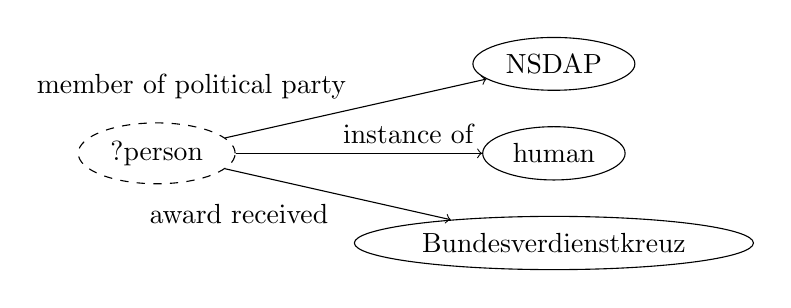
\begin{tikzpicture}
    \matrix[row sep=4mm] {
      & \node[iri] (NSDAP) {NSDAP}; \\
      \node[var] (person) {?person}; & \node[iri] (human) {human}; \\
      & \node[iri] (Bundesverdienstkreuz) {Bundesverdienstkreuz}; \\
    };
    \draw[predicate] (person) to node {member of political party} (NSDAP);
    \draw[predicate] (person) to node [pos=.7] {instance of} (human);
    \draw[predicate,swap] (person) to node {award received} (Bundesverdienstkreuz);
  \end{tikzpicture}
  \pause

  \begin{lstlisting}
    SELECT ?person WHERE {
      ?person wdt:P31 wd:Q5;
              wdt:P102 wd:Q7320;
              wdt:P166 wd:Q21164.
    }
  \end{lstlisting}
\end{frame}

\begin{frame}[fragile]
  \frametitle{Example queries}
  What are the largest cities (by population) with a female mayor?

  \begin{overprint}
    \onslide<2>
    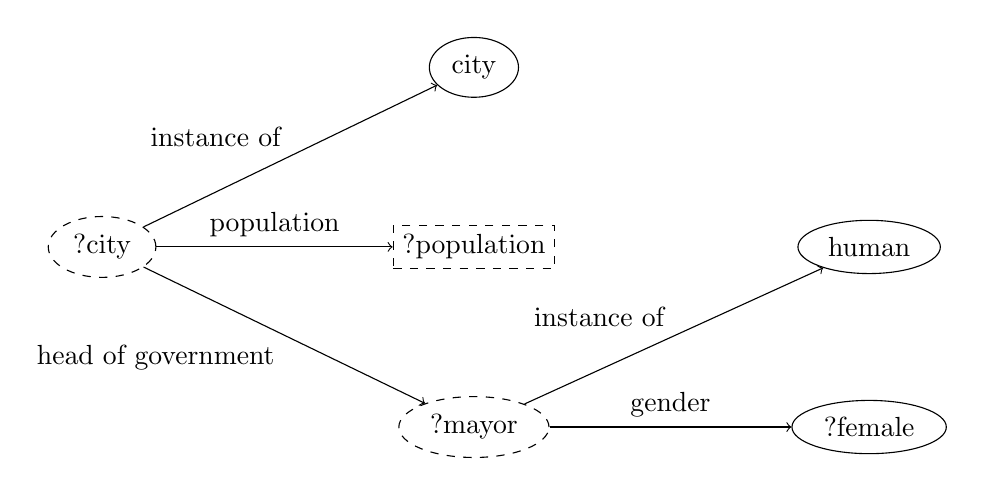
\begin{tikzpicture}
      \matrix[row sep=15mm,column sep=30mm] {
        & \node[iri] (City) {city}; & \\
        \node[var] (city) {?city}; & \node[varliteral] (population) {?population}; & \node[iri] (human) {human}; \\
        & \node[var] (mayor) {?mayor}; & \node[iri] (female) {?female}; \\
      };
      \draw[predicate] (city) to node {instance of} (City);
      \draw[predicate] (city) to node {population} (population);
      \draw[predicate,swap] (city) to node {head of government} (mayor);
      \draw[predicate] (mayor) to node {instance of} (human);
      \draw[predicate] (mayor) to node {gender} (female);
    \end{tikzpicture}

    (Not pictured: the “largest” part.)
  
    \onslide<3>
    \begin{lstlisting}
      SELECT ?city ?mayor ?population WHERE {
        ?city wdt:P31 wd:Q515;
              wdt:P1082 ?population;
              wdt:P6 ?mayor.
        ?mayor wdt:P31 wd:Q5;
               wdt:P21 wd:Q6581072.
      }
      ORDER BY DESC(?population)
      LIMIT 10
    \end{lstlisting}
    (Note that this misses some items that are e.\,g. “instance of: big city” rather than “instance of: city”.)
  
    \onslide<4>
    \begin{lstlisting}
      SELECT ?city WHERE {
        ?city wdt:P31 wd:Q515;
              wdt:P1082 ?population;
              wdt:P6 [
                wdt:P31 wd:Q5;
                wdt:P21 wd:Q6581072
              ].
      }
      ORDER BY DESC(?population)
      LIMIT 10
    \end{lstlisting}
  \end{overprint}
\end{frame}

\begin{frame}
  \frametitle{Closing stuff}
  \begin{itemize}
  \item Fun/interesting queries: \Twitter{WikidataFacts} or \Mastodon{WikidataFacts}{mastodon.social}
  \item Wikidata Query Service help portal: \href{https://www.wikidata.org/wiki/Special:MyLanguage/Wikidata:SPARQL_query_service/Wikidata_Query_Help}{wikidata:Help:SPARQL} (\wwiki{EV2})
  \item These slides: \href{https://github.com/lucaswerkmeister/36c3-wdqs}{github.com/lucaswerkmeister/36c3-wdqs}
  \item Other queries promised in the talk description:
    \begin{itemize}
    \item \href{https://www.wikidata.org/wiki/User:TweetsFactsAndQueries/Queries/films_starring_more_than_one_future_head_of_government}{Which films starred more than one future head of government?} (\wwiki{EV\$})
    \item \href{https://www.wikidata.org/wiki/User:TweetsFactsAndQueries/Queries/UK_parliaments_with_count_of_Johns_and_count_of_women}{When did women finally outnumber Johns in the House of Commons?} (\wwiki{EVz})
    \end{itemize}
  \end{itemize}
\end{frame}

\end{document}
